\section{Aufbau und Durchführung}

\begin{figure}[H]
  \centering
  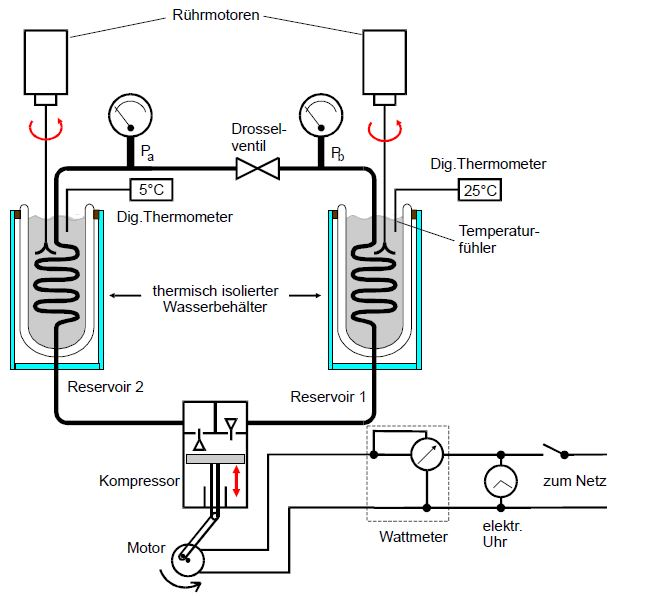
\includegraphics{Text/Bilder/WP2.jpg}
  \caption{Experimenteller Aufbau \cite[4]{sample}}
  \label{WP2}
\end{figure}
Die Reservoire 1 und 2 werden daraufhin mit einer
genau abgemessenen Wassermenge befüllt die gegebenen Daten zur Wärmekapazität notiert.
Daraufhin wird die Apperatur eingeschaltet. Die angezeigten Werte für $T_1$, $T_2$, $p_a$, $p_b$ und $N$ werden
im Minutentakt abgelesen und notiert.
Dies wird so lange gemacht, bis das Wasser in Reservoir 1 \SI{50}{°C} erreicht.
